%\clearpage\newpage

\section{Electron identification} 

Only 1/3 of the triggers during the initial data processing have reconstructed
negative tracks, and out of these only 1/2 are identified as containing an electron.
In this identification, there is still a pion contamination problem. 
The {\it candidate electron} of this analysis is the combination of 
\begin{itemize}
 \item Any reconstructed PART bank electron.
 \item Any reconstructed EVNT bank electron.
 \item Any negative unknown PART bank particle if there is no PART bank electron.
 \item Any negative unknown EVNT bank particle if there is no EVNT bank electron. 
\end{itemize}
\clearpage\newpage
There are 6 ID cuts defining a {\it good electron}
starting from a {\it candidate electron} based on its momentum $p$, its signal in the 
\v Cerenkov $nphe$, its signals in the forward calorimeter (total energy $EC_{tot}$, 
inner energy $EC_{in}$, outer energy $EC_{out}$) and its position on the EC $(x,y)$:
\begin{table}[h]
\begin{center}
  \begin{tabular}{l l}
$\bullet$  &  \v Cerenkov npe cut \\ &  \\
$\bullet$  & minimum $p$ cut \\&  \\
$\bullet$  & $EC_{tot} / p$ versus $p$ cut \\&  \\
$\bullet$  & $EC_{out}/p$ vs $EC_{in}/p$ cut \\&  \\
$\bullet$  & $EC_{in}$ / $EC_{tot}$ cut \\&  \\
$\bullet$  & $x_{_{EC}}$ vs $y_{_{EC}}$ cut \\&  \\
\end{tabular}
 \end{center}
\end{table}

Each cut is discussed below.

\subsection{\v Cerenkov signal cut}
\label{sec:cc_cut}
A threshold for the signal in the \v Cerenkov detector (CC) is necessary to eliminate electronic noise
and the fact that pions produce \v Cerenkov light when their momentum is above $\sim 2.5$ GeV.

The signal from the CC is amplified by 10 and converted in {\it number of photoelectrons} (nphe). 
Fig.\ref{fig:cccut} shows the cut used: 
\begin{center}
nphe $> 2.5$  
\end{center}
\begin{figure}[h]
\begin{center}
  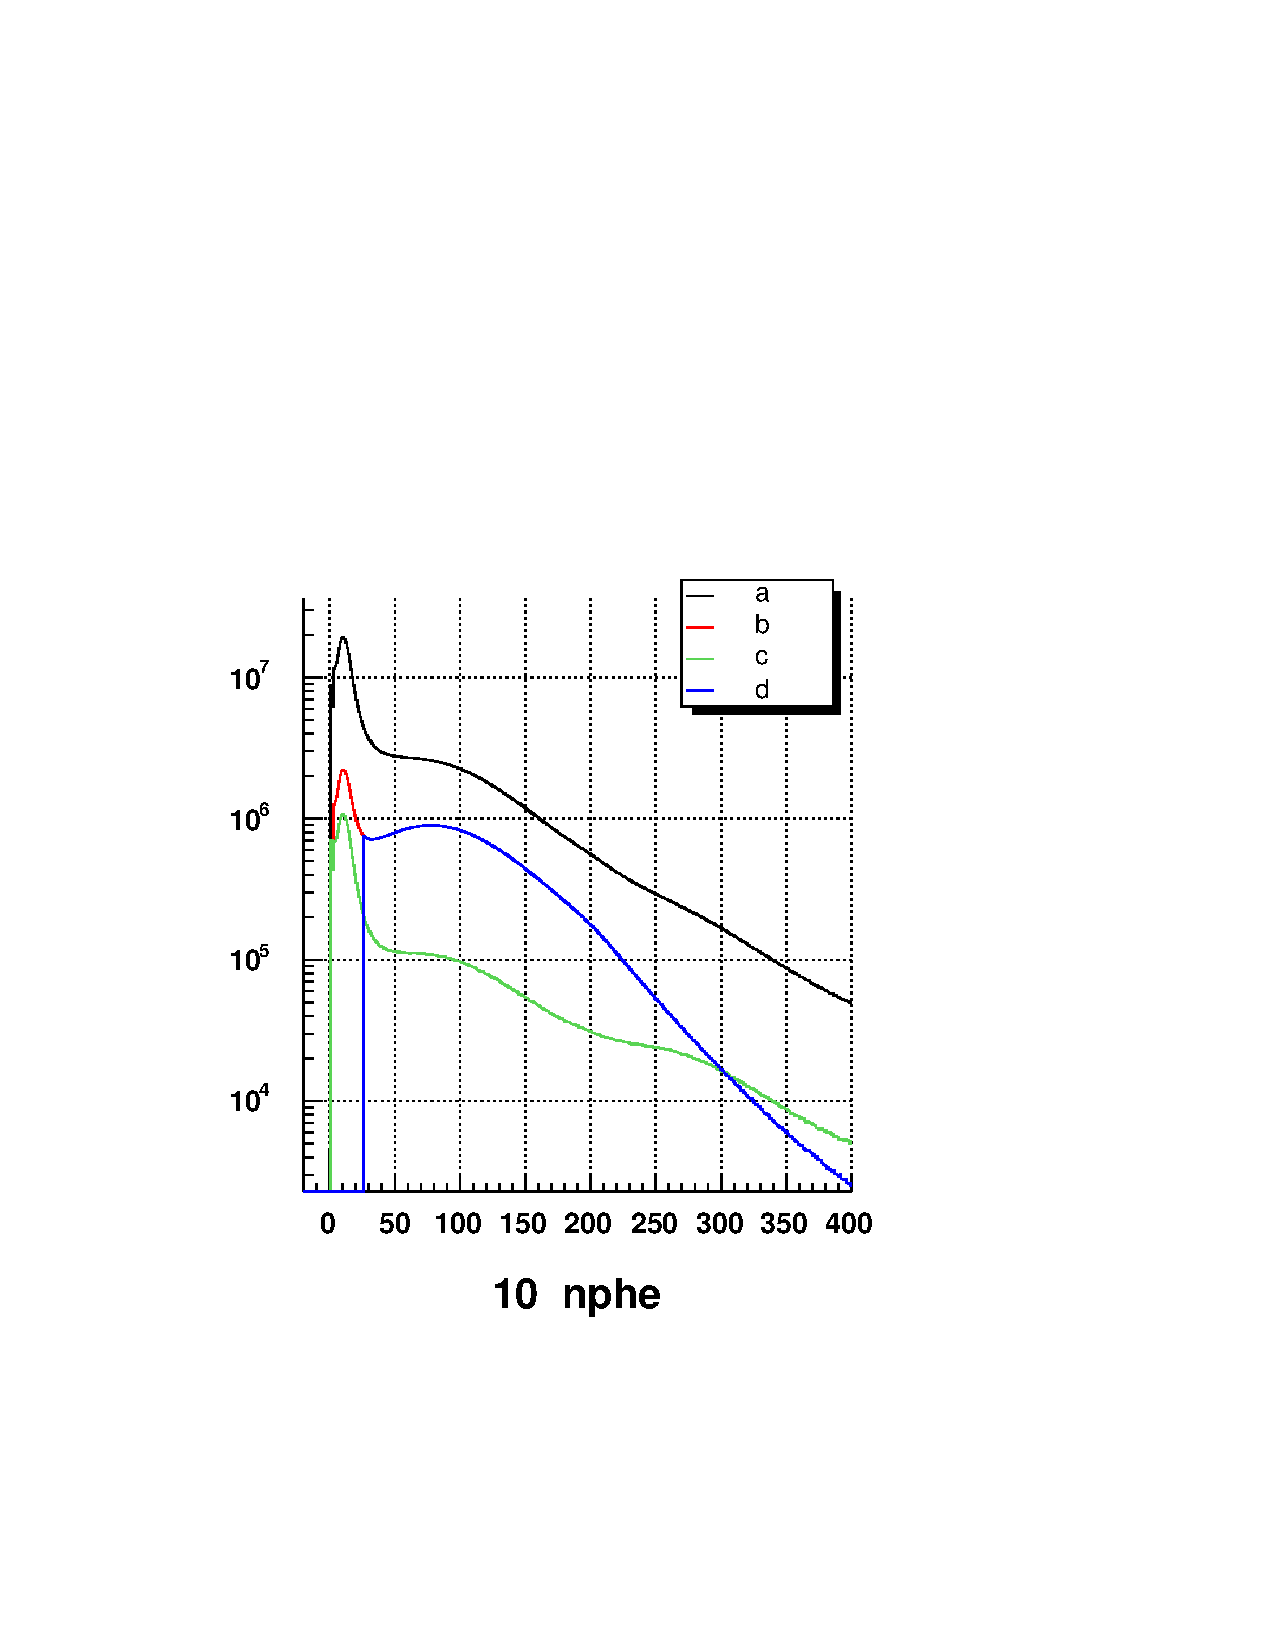
\includegraphics[width = 12cm, bb=50 140 500 540]{data_reduction/img/cc_pid}
  \caption[The CC signal threshold cut]
          { The CC signal threshold cut: 10 nphe.\\
	             (a) all electrons.
	             (b) electrons with all other ID cuts (aside from \v Cerenkov cut) applied. One can see that the 
	             signal at 100 ($\sim 10$ nphe) is enhanced while the noise at $nphe\sim 10$ is suppressed. 
		     (c) electrons with all other ID 
	             anti-cuts (aside from \v Cerenkov cut) applied. This events corresponds to the pions and the noise.
		     (d) electrons with all ID cuts applied.}
 \label{fig:cccut}
 \end{center}
\end{figure}

\subsection{Total energy in the calorimeter}
In the momentum range detected at CLAS, when going through the forward calorimeter
charged pions are minimum ionizing particles, while electrons shower with a total energy 
deposition $E_{tot}$ proportional to their momentum $P$. 
Hence $E_{tot}/P$ should be constant. In reality this ratio shows a slight momentum dependance as
it is illustrated in \F{fig:ec1cut} where 
the $E_{tot}/P$ distribution is plotted versus $P$.
This distribution was sliced along $P$ and each slice is
fitted with a gaussian distribution, giving the mean and sigma as a function
of $p$:
$$
\begin{array}{l}
\bar{p} = \bar{p}(p) \\
\sigma = \sigma (p)
\end{array}
$$
A second order polynomial is fitted to those distributions and
events are accepted if they occur within 3 $\sigma$  around $\bar{p}$, i.e. if
$$
 \bar{p} - 3\sigma \,\le\, E_{tot}/P \,\le\, \bar{p} + 3\sigma
$$
The cut is shown in \F{fig:ec1cut} as dotted red lines. The function is reported in \ref{sec:ectotvsp}.

\subsection{ Minimum $p$ cut}
A study \cite{bib:ecmin} of the inclusive cross section at various beam energies in CLAS 
results in a low momentum cut $p_{min}$ depending on the calorimeter low total threshold
(in milliVolts)
of the trigger discriminator:
$$
 p_{min}\,\,{\rm (MeV)} = 214 + 2.47\times EC_{threshold}{\rm (mV)}
$$
The threshold for e1-6 was $172$ mV therefore the minimum momentum cut is fixed at:
$$
p_{min} = 0.64\,\,{\rm GeV}
$$
The cut is shown in \F{fig:ec1cut} as a vertical line.
\begin{figure}[t]
\begin{center}
  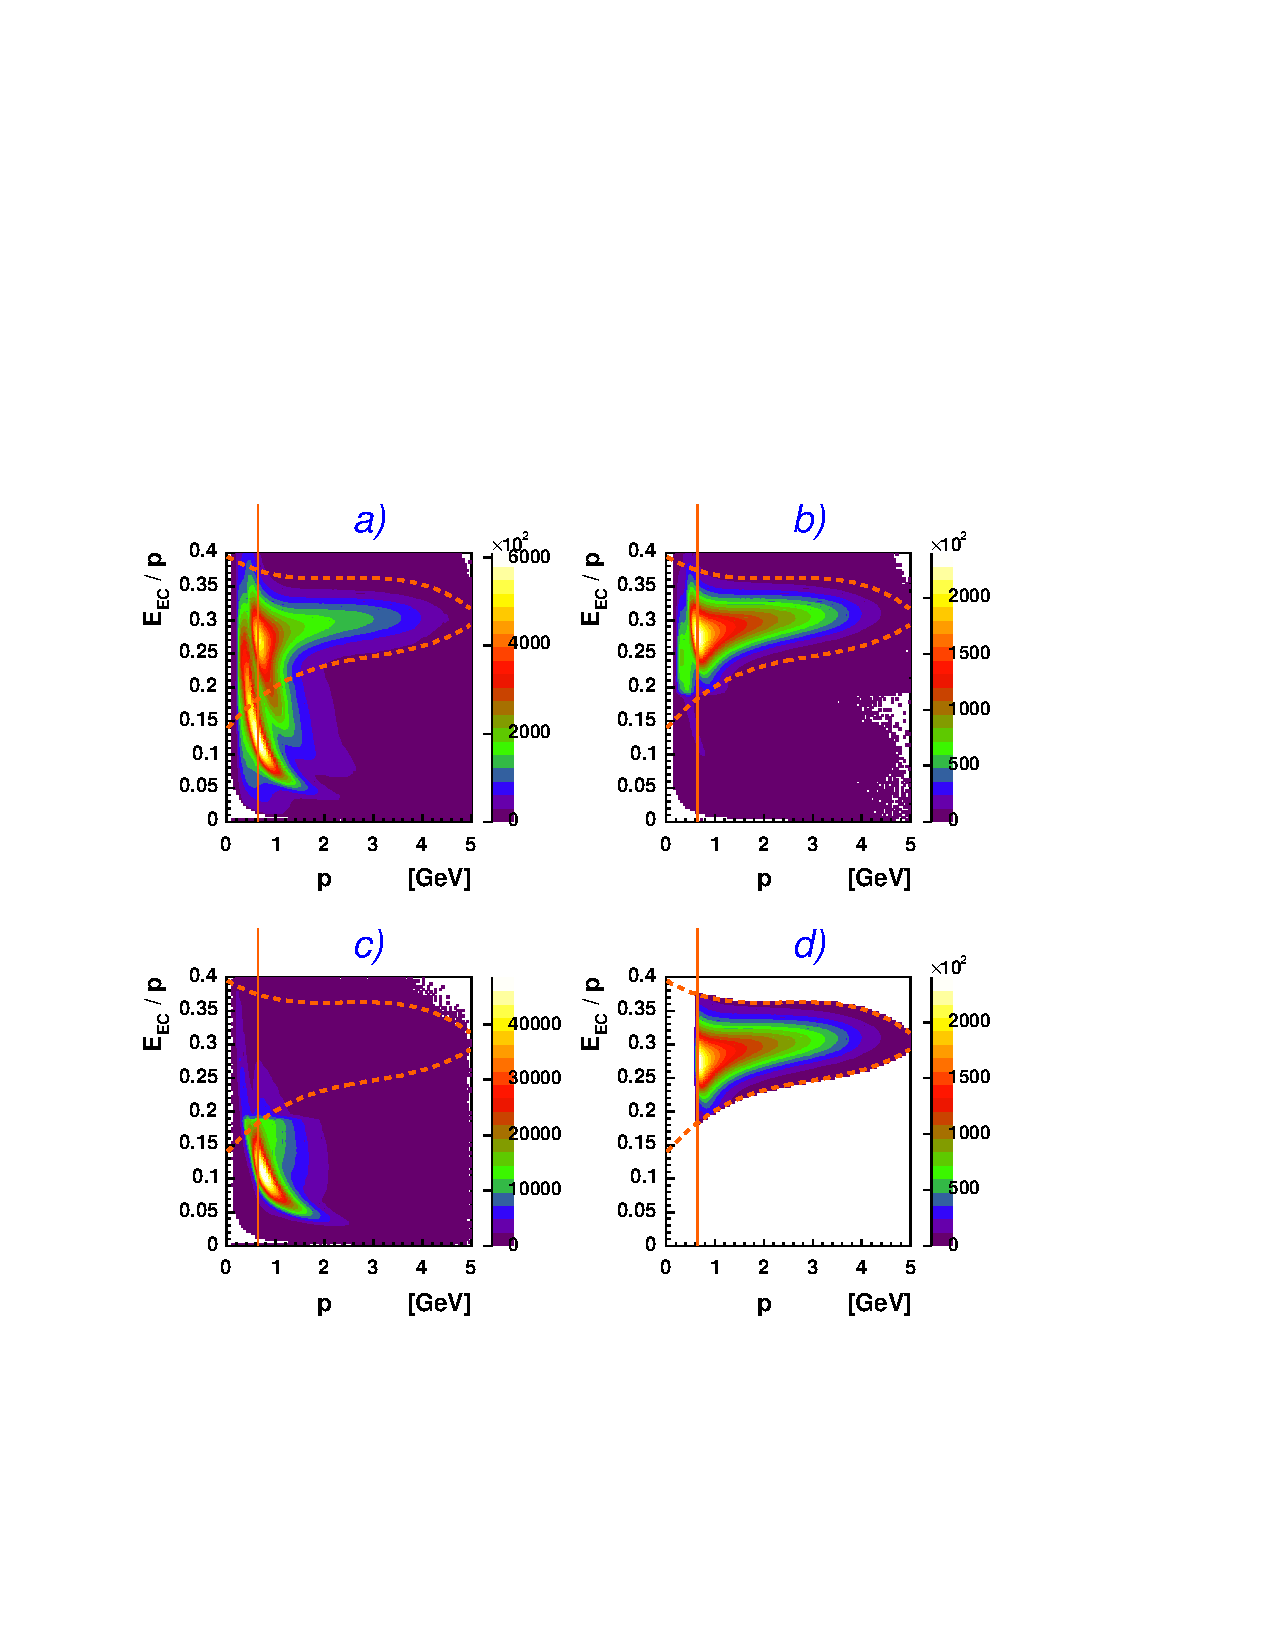
\includegraphics[width=11cm, bb=40 140 490 540]{data_reduction/img/ec1_pid}
  \caption[$E_{tot}$ and $p_{min}$ cut]
  { $E_{tot}$ and $p_{min}$ cut.
  	     For minimum ionizing particles $E_{tot}$ is constant so 
	     they show as an hyperbole.
             The vertical line represents the $p_{min}$ cut.
             The remaining two dashed lines are the $\bar{p} \pm 3\sigma$ cuts.
             (a) all electrons.
	     (b) electrons with all other ID cuts (aside from $E_{tot}$ and $p_{min}$ cuts) applied. 
             The band corresponding to minimum ionizing particles disappears almost completely.
             (c) electrons with all other ID 
	     anti-cuts (aside from $E_{tot}$ and $p_{min}$ cuts) applied. 
	     These events correspond to minimum ionizing particles and background.
             (d) electrons with all ID cuts applied.}
 \label{fig:ec1cut}
 \end{center}
\end{figure}
\cia\vspace{-2cm}
\subsection{  $EC_{out}/p$ vs $EC_{in}/p$ cut}
The outer EC is $5/3$ times larger than the inner EC. Therefore pions, 
which do not shower and are minimum ionizing,  
release a small quantity of energy in the outer and inner part in the ratio $5:3$.
On the other hand 
electrons release a lot more energy because they shower. 
Due to the shower geometry electrons
release more energy in the inner part than in the outer part.

The quantity $E_{in}/p$ is plotted versus $E_{out}/p$ in \F{fig:ec2cut}.
One can see the pions along the cyan line $y=\Dfrac{5}{3}\,x$ and the electrons
on the right part of the red line, which represents the cut and assumes the form
$$
 y = 0.19 - x
$$

A bug in the reconstruction code sometimes gives a wrong (zero) values for $E_{in}$, $E_{out}$. For
those events, this cut was not applied.

\subsection{ $E_{in} / E_{out}$ cut}
Electrons
release more energy in the inner part of the calorimeter than in the outer part because
of the shower conformation. This can be seen in \F{fig:ec3cut} where $E_{in} / E_{out}$ is
plotted against $p$. 

By looking at the plot, a low threshold cut on $E_{in} / E_{TOT}$ is introduced at $40\%$:
$$
 E_{in} / E_{TOT} \ge 0.4
$$
The cut is shown in the figure as an horizontal red line.



\begin{figure}[h]
\begin{center}
  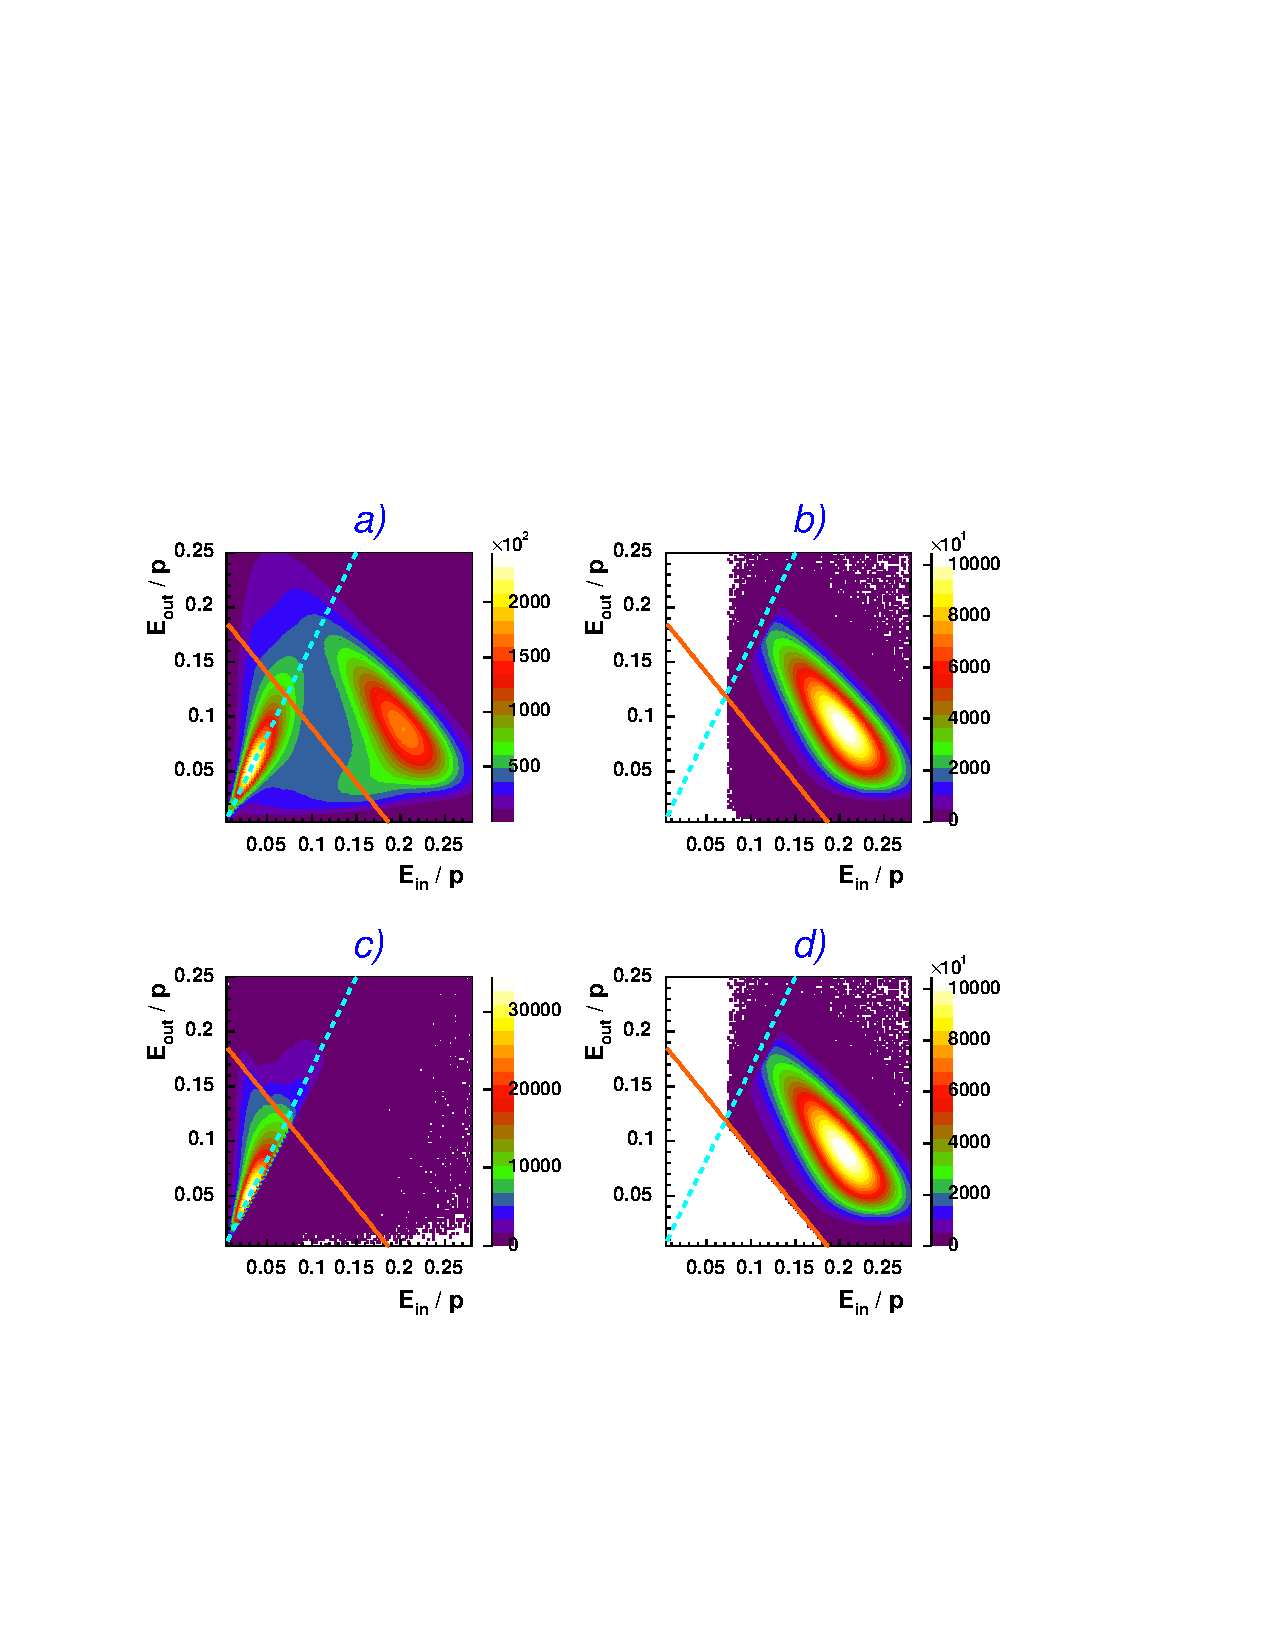
\includegraphics[width=12cm, bb=50 140 490 580]{data_reduction/img/ec2_pid}
  \caption[$EC_{out}/p$ vs $EC_{in}/p$ cut]
          { $EC_{out}/p$ vs $EC_{in}/p$ cut.
	     (a) all electrons.
	     (b) electrons with all other ID cuts (aside from $EC_{out}/p$ vs $EC_{in}/p$ cut) applied. 
             The band corresponding to minimum ionizing particles disappears almost completely.
             (c) electrons with all other ID 
	     anti-cuts (aside from $EC_{out}/p$ vs $EC_{in}/p$ cut) applied. 
	     This events corresponds to minimum ionizing particles and background.
             (d) electrons with all ID cuts applied.}
 \label{fig:ec2cut}
  \end{center}
\end{figure}


\begin{figure}[h]
\begin{center}
  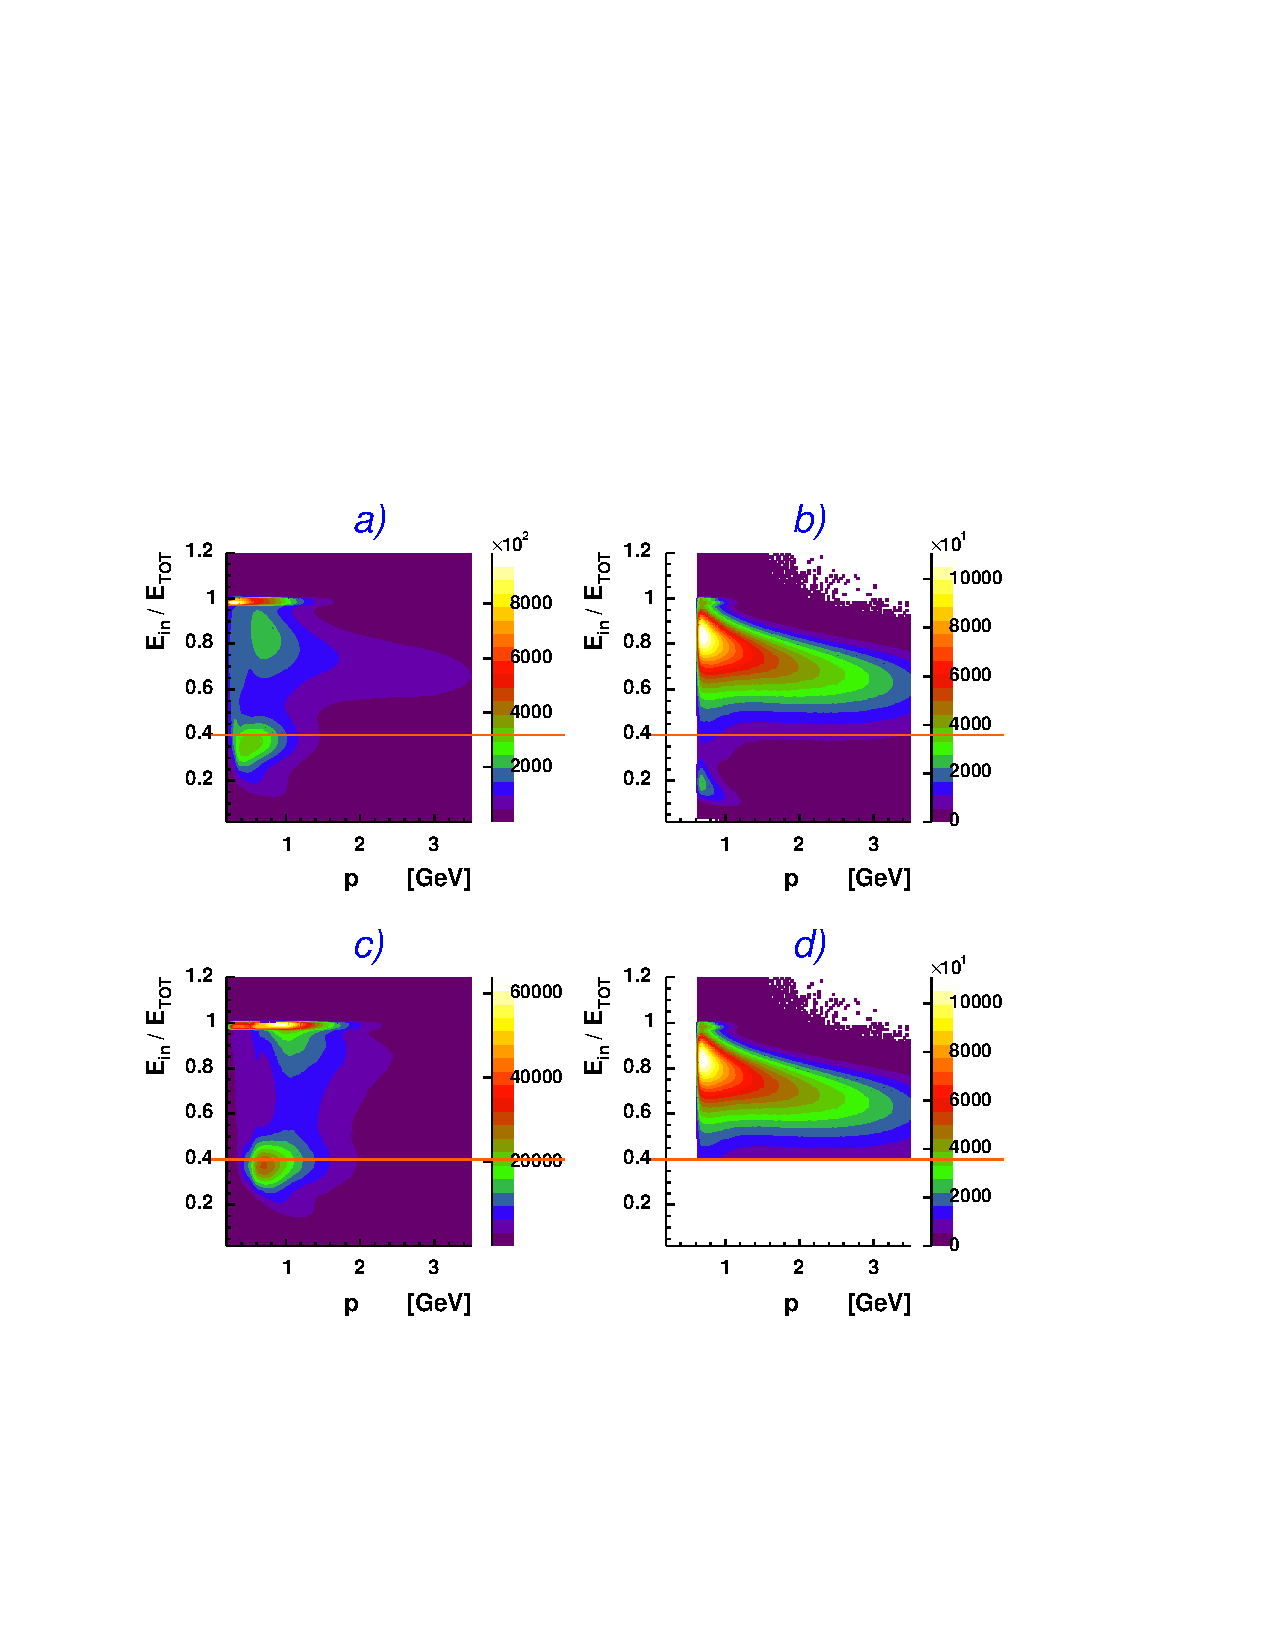
\includegraphics[width=12cm, bb=60 120 490 560]{data_reduction/img/ec3_pid}
  \caption[ The $E_{in}/E_{tot}$ cut.]
          { The $E_{in}/E_{tot}$ cut. Particles that are stopped in the inner part (hence
	             have small energy) have $E_{in} = E_{tot}$ so they show up at  $E_{in}/E_{tot}=1$.
		     Most of these are cut out with the ID cuts.		   
	             (a) all electrons.
		     (b) electrons with all other ID cuts (aside from $E_{in}/E_{tot}$ cut) applied. 
       	      	     (c) electrons with all other ID 
		     anti-cuts (aside from $E_{in}/E_{tot}$  cut) applied. 		      
                     Minimum ionizing particles are enhanced here. They release comparable 
		     energy in the inner and outer part. Since the inner part is $3/8$ of the 
		     total calorimeter, they peak in this plot at $3/8=0.375\%$.
                     (d) electrons with all ID cuts applied.}	  
 \label{fig:ec3cut}
 \end{center}
\end{figure}

\subsection{Track position cut}
Electrons that shower near the edges of the calorimeter will not loose
all their energy in the detector because the shower is truncated.
Hence their energy cannot be properly reconstructed.

For this reason a fiducial cut is introduced on the track coordinates $x,y$ of the electrons 
at the EC plane. The cut is illustrated in \F{fig:ec4cut}.

\begin{figure}[h]
\begin{center}
  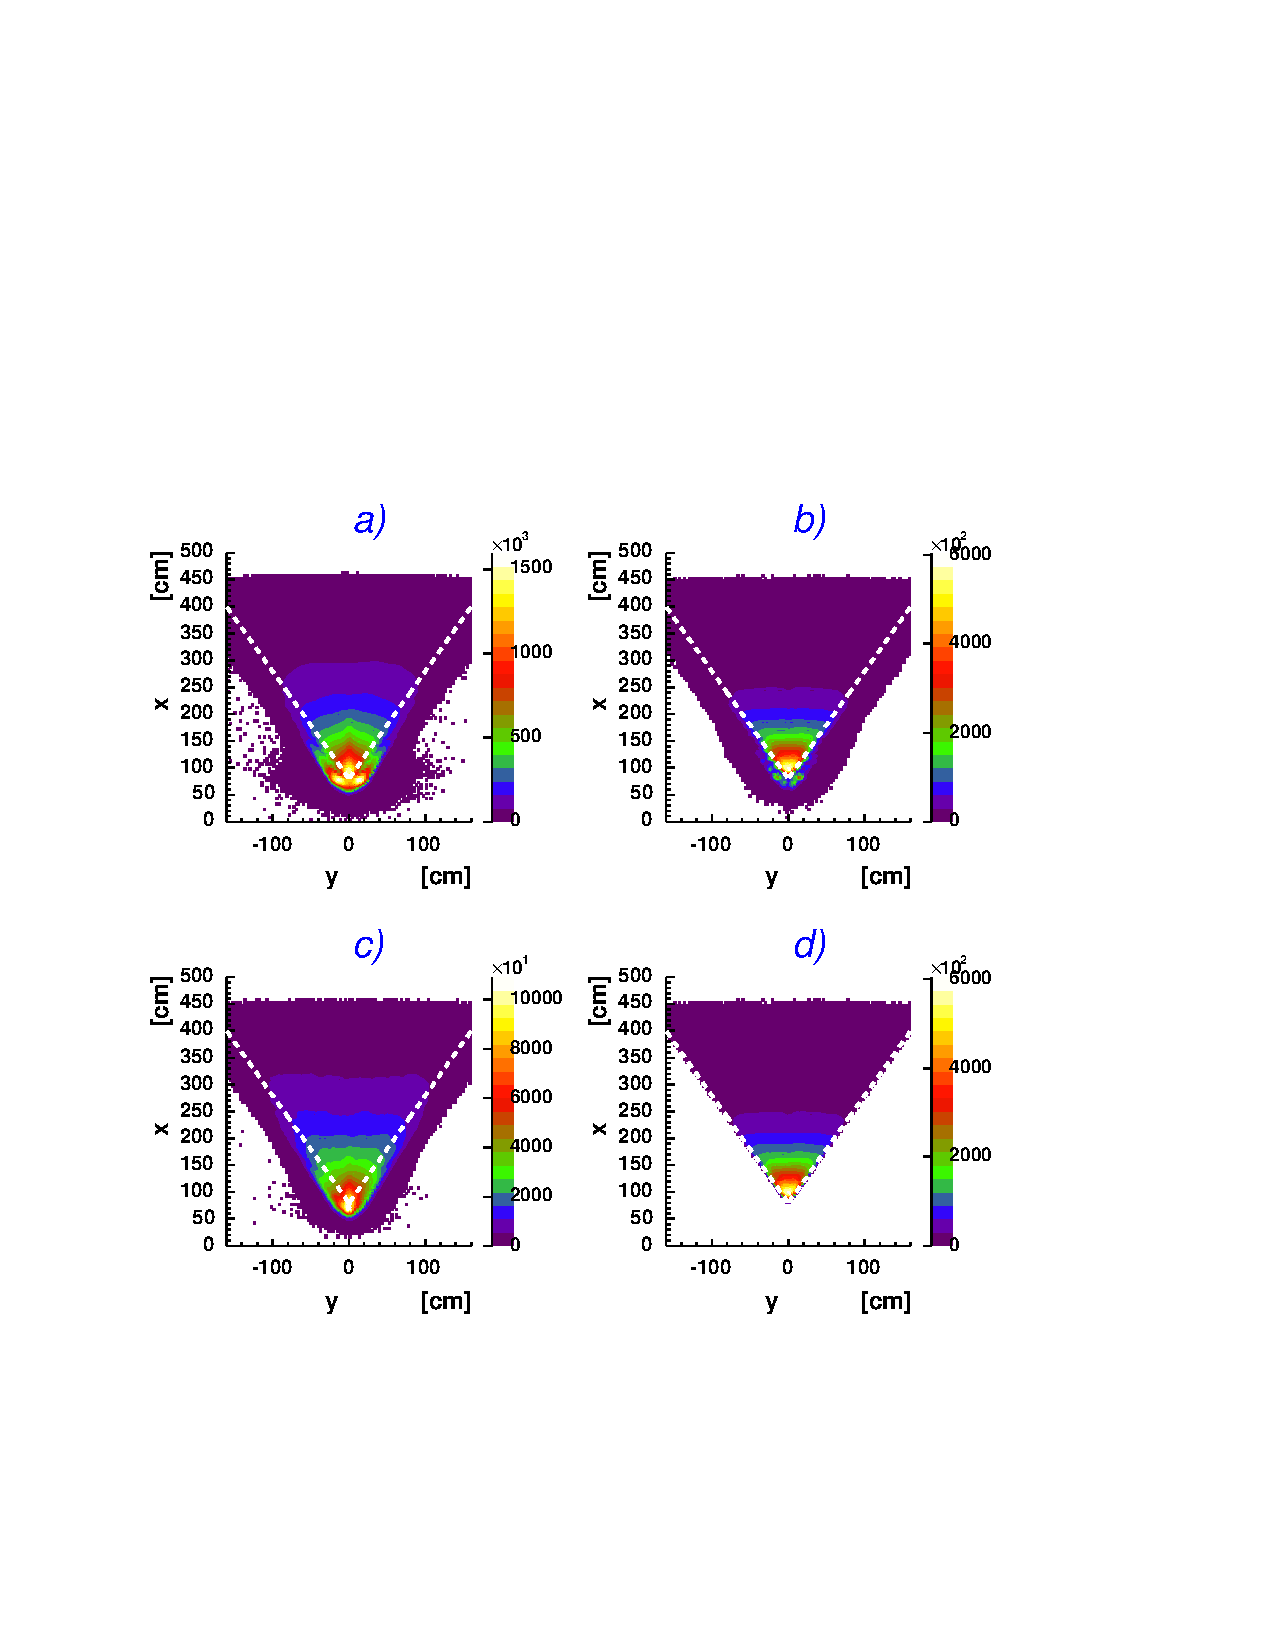
\includegraphics[width=12cm, bb=60 120 490 580]{data_reduction/img/ec4_pid}
  \caption[Track coordinates $(x,y)$ cut ]
          { Track coordinates $(x, y)$ cut. 
	             (a) all electrons.
		     (b) electrons with all other ID cuts (aside from $E_{in}/E_{tot}$ cut) applied. 
		     The $x,y$ cut is chosen so that it encompass the electrons in this plot.
       	      	     (c) electrons with all other ID 
		     anti-cuts (aside from $E_{in}/E_{tot}$  cut) applied. 		      
                     (d) electrons with all ID cuts applied.}	  	             
 \label{fig:ec4cut}
  \end{center}
\end{figure}














